\documentclass[11pt,a4paper]{article}
%%%%%%%%%%%%%%%%%%%%%%%%% Credit %%%%%%%%%%%%%%%%%%%%%%%%

% template ini dibuat oleh martin.manullang@if.itera.ac.id untuk dipergunakan oleh seluruh sivitas akademik itera.

%%%%%%%%%%%%%%%%%%%%%%%%% PACKAGE starts HERE %%%%%%%%%%%%%%%%%%%%%%%%
\usepackage{graphicx}
\usepackage{caption}
\usepackage{microtype}
\usepackage{lmodern}
\captionsetup[table]{name=Tabel}
\captionsetup[figure]{name=Gambar}
\usepackage{tabulary}
\usepackage{minted}
\usepackage{amsmath}
\usepackage{fancyhdr}
\usepackage{amssymb}
\usepackage{amsthm}
\usepackage{placeins}
\usepackage{amsfonts}
\usepackage{graphicx}
\usepackage[all]{xy}
\usepackage{tikz}
\usepackage{verbatim}
\usepackage[left=2cm,right=2cm,top=3cm,bottom=2.5cm]{geometry}
\usepackage{hyperref}
\hypersetup{
    colorlinks,
    linkcolor={red!50!black},
    citecolor={blue!50!black},
    urlcolor={blue!80!black}
}
\usepackage{caption}
\usepackage{subcaption}
\usepackage{multirow}
\usepackage{psfrag}
\usepackage[T1]{fontenc}
% \usepackage[scaled]{beramono} % Disabled to avoid pdfTeX font expansion error
% Enable inserting code into the document
\usepackage{listings}
\usepackage{xcolor} 
% custom color & style for listing
\definecolor{codegreen}{rgb}{0,0.6,0}
\definecolor{codegray}{rgb}{0.5,0.5,0.5}
\definecolor{codepurple}{rgb}{0.58,0,0.82}
\definecolor{backcolour}{rgb}{0.95,0.95,0.92}
\definecolor{LightGray}{gray}{0.9}
\lstdefinestyle{mystyle}{
	backgroundcolor=\color{backcolour},   
	commentstyle=\color{green},
	keywordstyle=\color{codegreen},
	numberstyle=\tiny\color{codegray},
	stringstyle=\color{codepurple},
	basicstyle=\ttfamily\footnotesize,
	breakatwhitespace=false,         
	breaklines=true,                 
	captionpos=b,                    
	keepspaces=true,                 
	numbers=left,                    
	numbersep=5pt,                  
	showspaces=false,                
	showstringspaces=false,
	showtabs=false,                  
	tabsize=2
}
\lstset{style=mystyle}
\renewcommand{\lstlistingname}{Kode}
%%%%%%%%%%%%%%%%%%%%%%%%% PACKAGE ends HERE %%%%%%%%%%%%%%%%%%%%%%%%


%%%%%%%%%%%%%%%%%%%%%%%%% Data Diri %%%%%%%%%%%%%%%%%%%%%%%%
\newcommand{\student}{\textbf{Dina Rahma Dita (122140184)}}
\newcommand{\course}{\textbf{Sistem Teknologi Multimedia (IF25-40305)}}
\newcommand{\assignment}{\textbf{Worksheet 1: Setup Python Environment untuk Multimedia}}

%%%%%%%%%%%%%%%%%%% using theorem style %%%%%%%%%%%%%%%%%%%%
\newtheorem{thm}{Theorem}
\newtheorem{lem}[thm]{Lemma}
\newtheorem{defn}[thm]{Definition}
\newtheorem{exa}[thm]{Example}
\newtheorem{rem}[thm]{Remark}
\newtheorem{coro}[thm]{Corollary}
\newtheorem{quest}{Question}[section]
%%%%%%%%%%%%%%%%%%%%%%%%%%%%%%%%%%%%%%%%
\usepackage{lipsum}%% a garbage package you don't need except to create examples.
\usepackage{fancyhdr}
\pagestyle{fancy}
\lhead{Dina Rahma Dita (122140184)}
\rhead{ \thepage}
\cfoot{\textbf{Worksheet 1: Setup Python Environment untuk Multimedia}}
\renewcommand{\headrulewidth}{0.4pt}
\renewcommand{\footrulewidth}{0.4pt}

%%%%%%%%%%%%%%  Shortcut for usual set of numbers  %%%%%%%%%%%

\newcommand{\N}{\mathbb{N}}
\newcommand{\Z}{\mathbb{Z}}
\newcommand{\Q}{\mathbb{Q}}
\newcommand{\R}{\mathbb{R}}
\newcommand{\C}{\mathbb{C}}
\setlength\headheight{14pt}

%%%%%%%%%%%%%%%%%%%%%%%%%%%%%%%%%%%%%%%%%%%%%%%%%%%%%%%555
\begin{document}

\thispagestyle{empty}
\begin{center}
	
\includegraphics[scale = 0.15]{Figure/ifitera-header.png}
	\vspace{0.1cm}
\end{center}
\noindent
\rule{17cm}{0.2cm}\\[0.3cm]
Nama: \student \hfill Tugas Ke: \assignment\\[0.1cm]
Mata Kuliah: \course \hfill Tanggal: \today\\
\rule{17cm}{0.05cm}
\vspace{0.1cm}



%%%%%%%%%%%%%%%%%%%%%%%%%%%%%%%%%%%%%%%%%%%%% BODY DOCUMENT %%%%%%%%%%%%%%%%%%%%%%%%%%%%%%%%%%%%%%%%%%%%%
\section{Tujuan Pembelajaran}
Setelah menyelesaikan worksheet ini, mahasiswa diharapkan mampu:
\begin{itemize}
    \item Memahami pentingnya manajemen environment Python untuk pengembangan multimedia
    \item Menginstall dan mengkonfigurasi Python environment menggunakan conda, venv, atau uv
    \item Menginstall library-library Python yang diperlukan untuk multimedia processing
    \item Memverifikasi instalasi dengan mengimpor dan menguji library multimedia
    \item Mendokumentasikan proses konfigurasi dan hasil pengujian dalam format \LaTeX
\end{itemize}

\section{Latar Belakang}
Python telah menjadi bahasa pemrograman yang sangat populer untuk multimedia processing karena memiliki ekosistem library yang sangat kaya. Namun, untuk dapat bekerja dengan multimedia secara efektif, kita perlu mengatur environment Python dengan benar dan menginstall library-library yang tepat.

Manajemen environment Python sangat penting untuk:
\begin{itemize}
    \item Menghindari konflik antar library (dependency conflict)
    \item Memastikan reproducibility dari project
    \item Memudahkan kolaborasi antar developer
    \item Memisahkan project yang berbeda dengan requirement yang berbeda
\end{itemize}

\section{Instruksi Tugas}

\subsection{Persiapan}
\textbf{Sebelum memulai, pastikan Anda telah:}
\begin{itemize}
    \item Menginstall Python 3.8 atau lebih baru di sistem Anda
    \item Memilih salah satu tool manajemen environment: \textbf{conda}, \textbf{venv}, atau \textbf{uv}
    \item Membuka terminal/command prompt
    \item Menyiapkan dokumen \LaTeX\ ini untuk dokumentasi
\end{itemize}

\subsection{Bagian 1: Membuat Environment Python}
Pilih \textbf{SALAH SATU} dari tiga opsi berikut dan ikuti langkah-langkahnya:

\subsubsection{Opsi 1: Menggunakan Conda (Direkomendasikan untuk pemula)}
Jalankan perintah berikut di terminal:

\begin{lstlisting}[language=bash, caption=Membuat environment dengan Conda]
# Membuat environment baru dengan nama 'multimedia'
conda create -n multimedia python=3.11

# Mengaktifkan environment
conda activate multimedia

# Verifikasi environment aktif
conda info --envs
\end{lstlisting}

\subsubsection{Opsi 2: Menggunakan venv (Built-in Python)}
\begin{lstlisting}[language=bash, caption=Membuat environment dengan venv]
# Membuat environment baru
python3 -m venv multimedia-env

# Mengaktifkan environment (Linux/Mac)
source multimedia-env/bin/activate

# Mengaktifkan environment (Windows)
# multimedia-env\Scripts\activate

# Verifikasi environment aktif
which python
\end{lstlisting}

\subsubsection{Opsi 3: Menggunakan uv (Modern dan cepat)}
\begin{lstlisting}[language=bash, caption=Membuat environment dengan uv]
# Install uv terlebih dahulu jika belum ada
# pip install uv

# Membuat environment baru
uv venv multimedia-uv

# Mengaktifkan environment (Linux/Mac)
source multimedia-uv/bin/activate

# Mengaktifkan environment (Windows)
# multimedia-uv\Scripts\activate

# Verifikasi environment aktif
which python
\end{lstlisting}

\textbf{Dokumentasikan di sini:}
\begin{itemize}
    \item Tool manajemen environment yang Anda pilih: \textbf{[Conda]}
    \item Screenshot atau copy-paste output dari perintah verifikasi environment
\end{itemize}

\begin{figure}[h!]
    \centering
    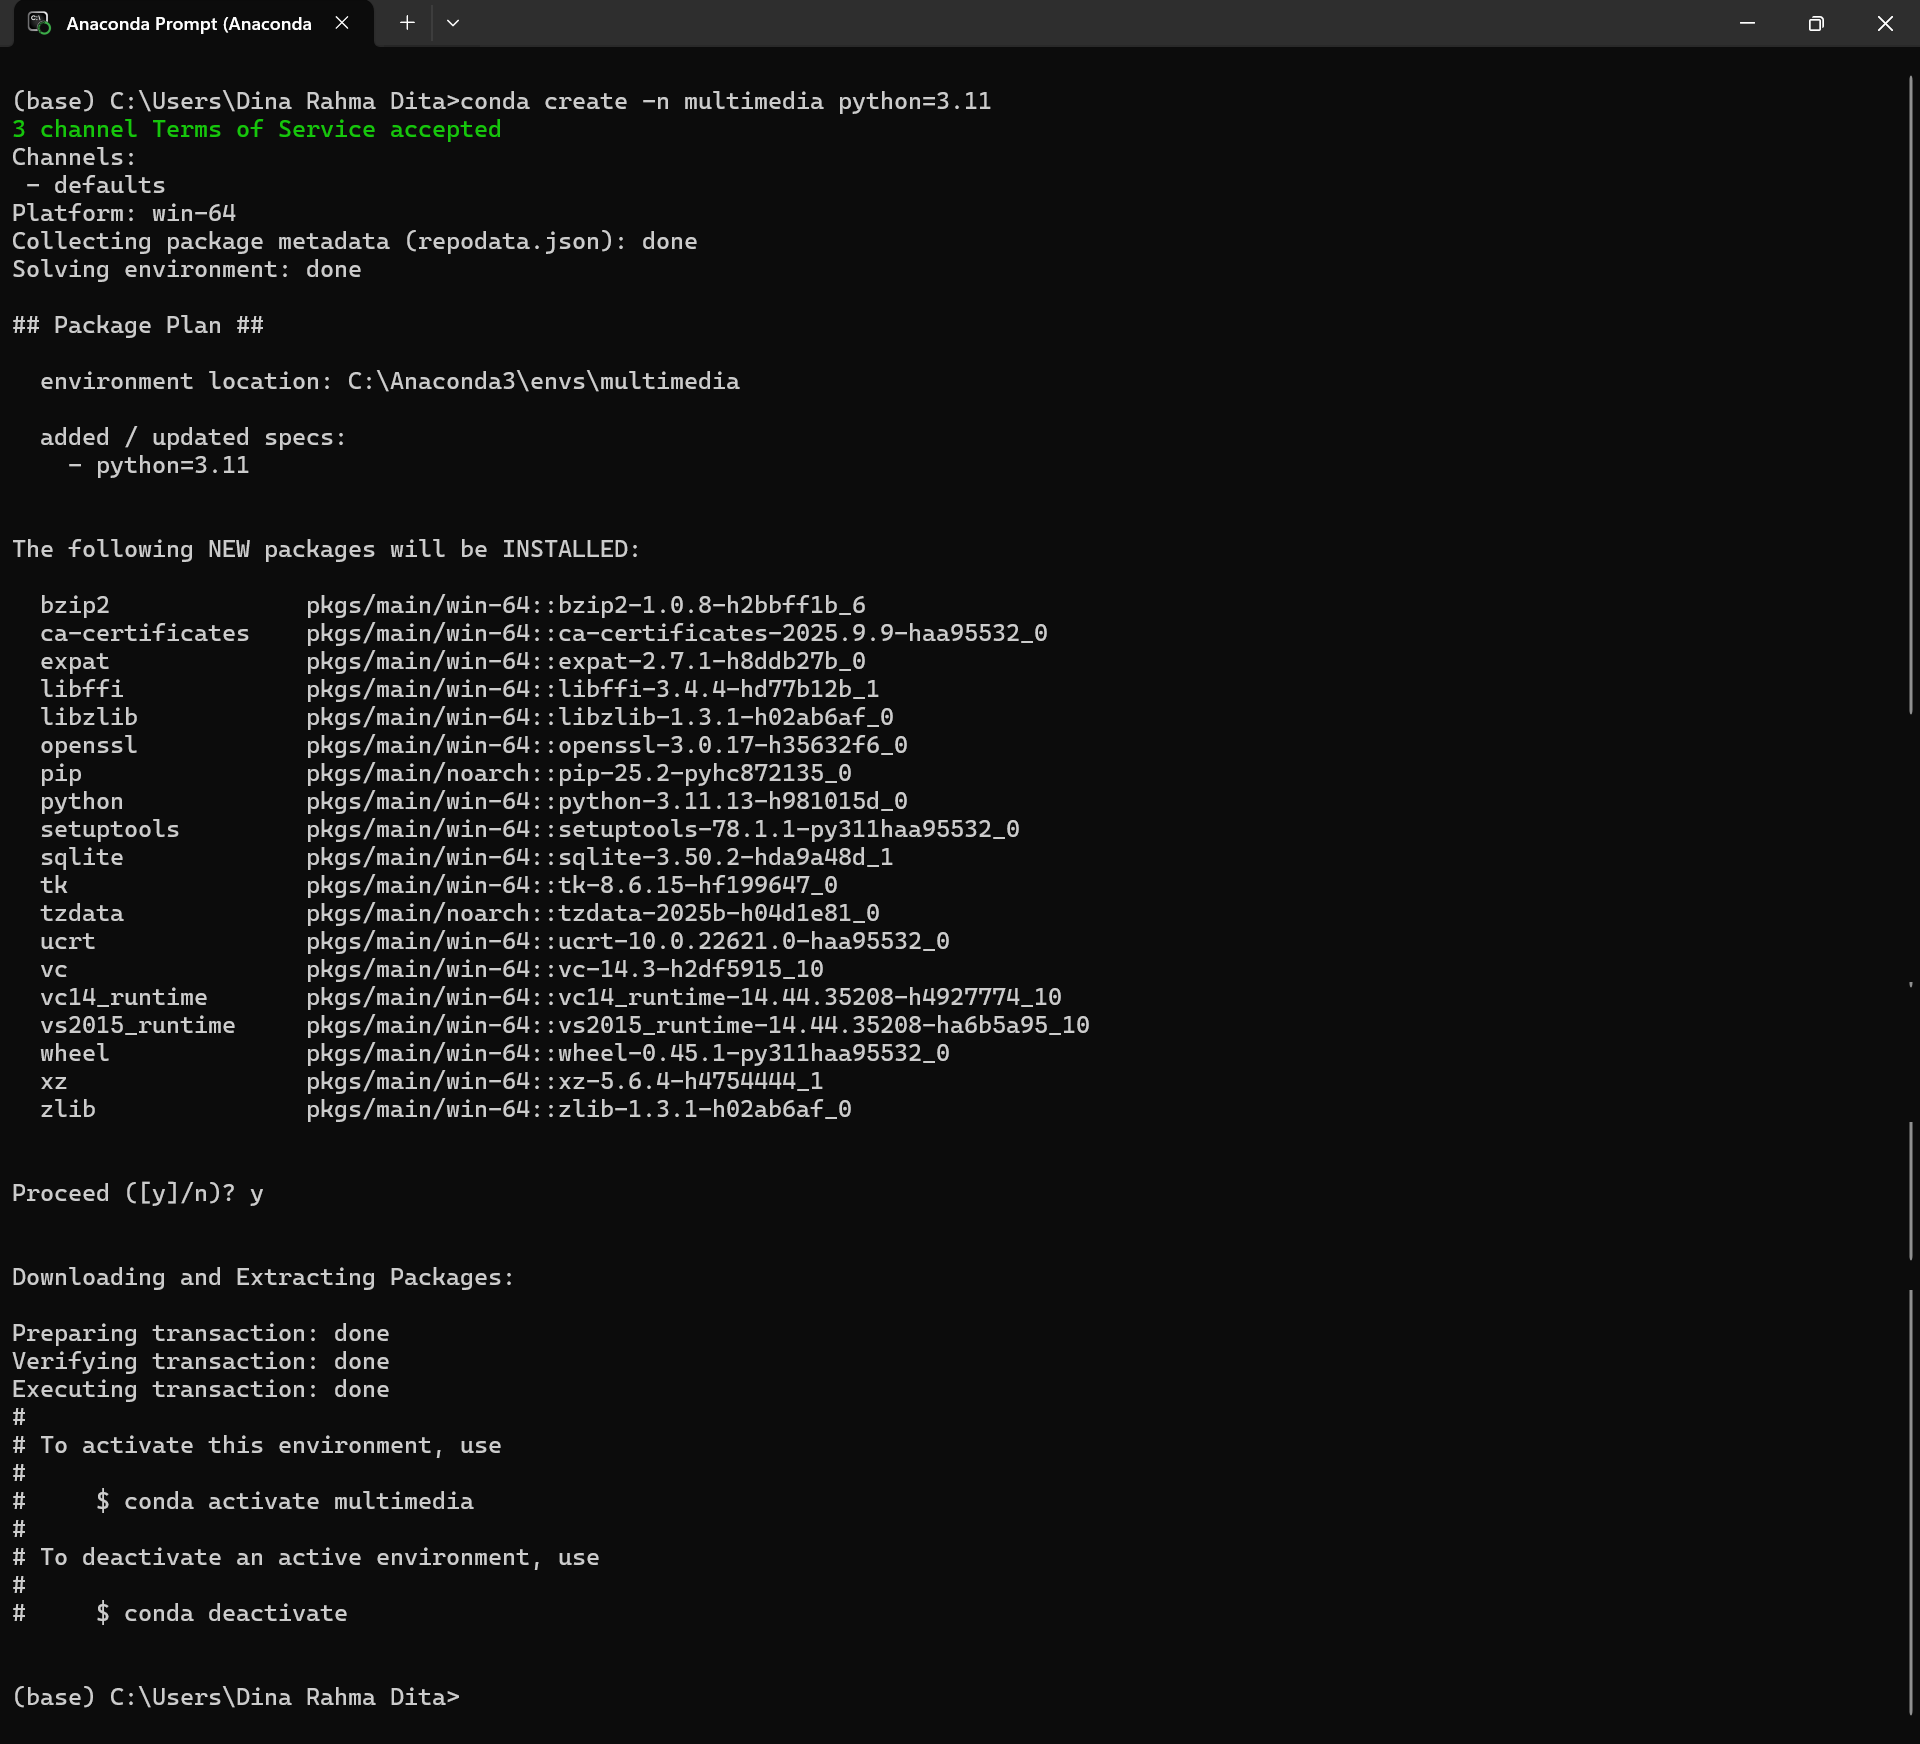
\includegraphics[width=0.8\textwidth]{Figure/ss/1.png}
    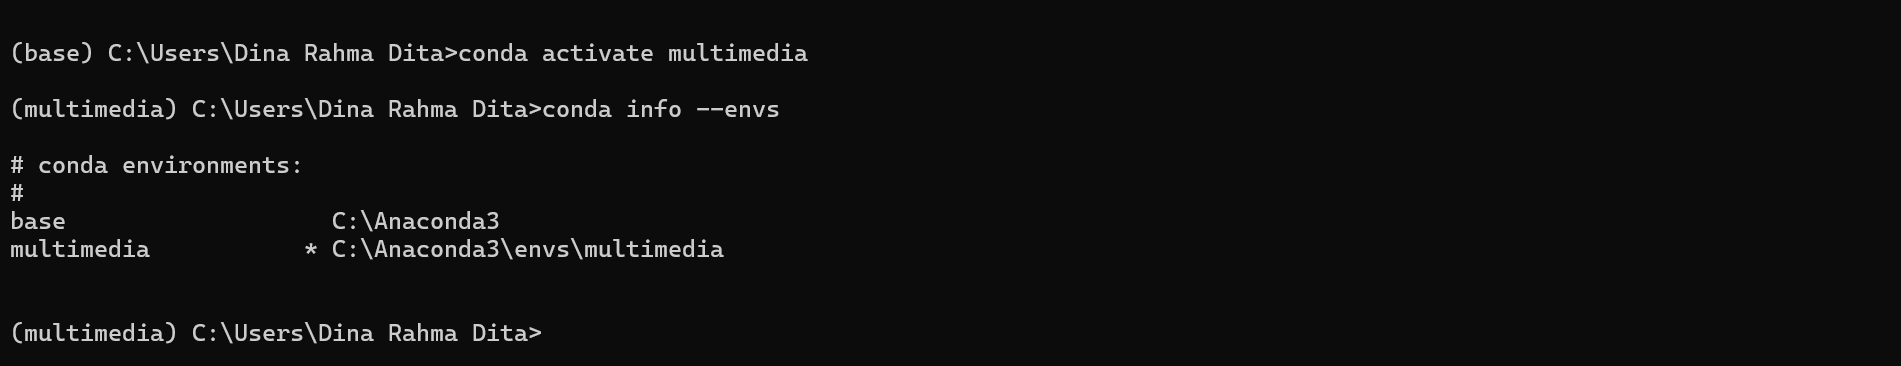
\includegraphics[width=0.8\textwidth]{Figure/ss/2.png}
    \caption{Hasil verifikasi environment dengan conda}
    \label{fig:test_env}
\end{figure}

\subsection{Bagian 2: Instalasi Library Multimedia}
Setelah environment aktif, install library-library berikut:

\subsubsection{Library Audio Processing}
\begin{lstlisting}[language=bash, caption=Instalasi library audio]
# Untuk conda:
conda install -c conda-forge librosa soundfile scipy
\end{lstlisting}

\begin{figure}[H]
    \centering
    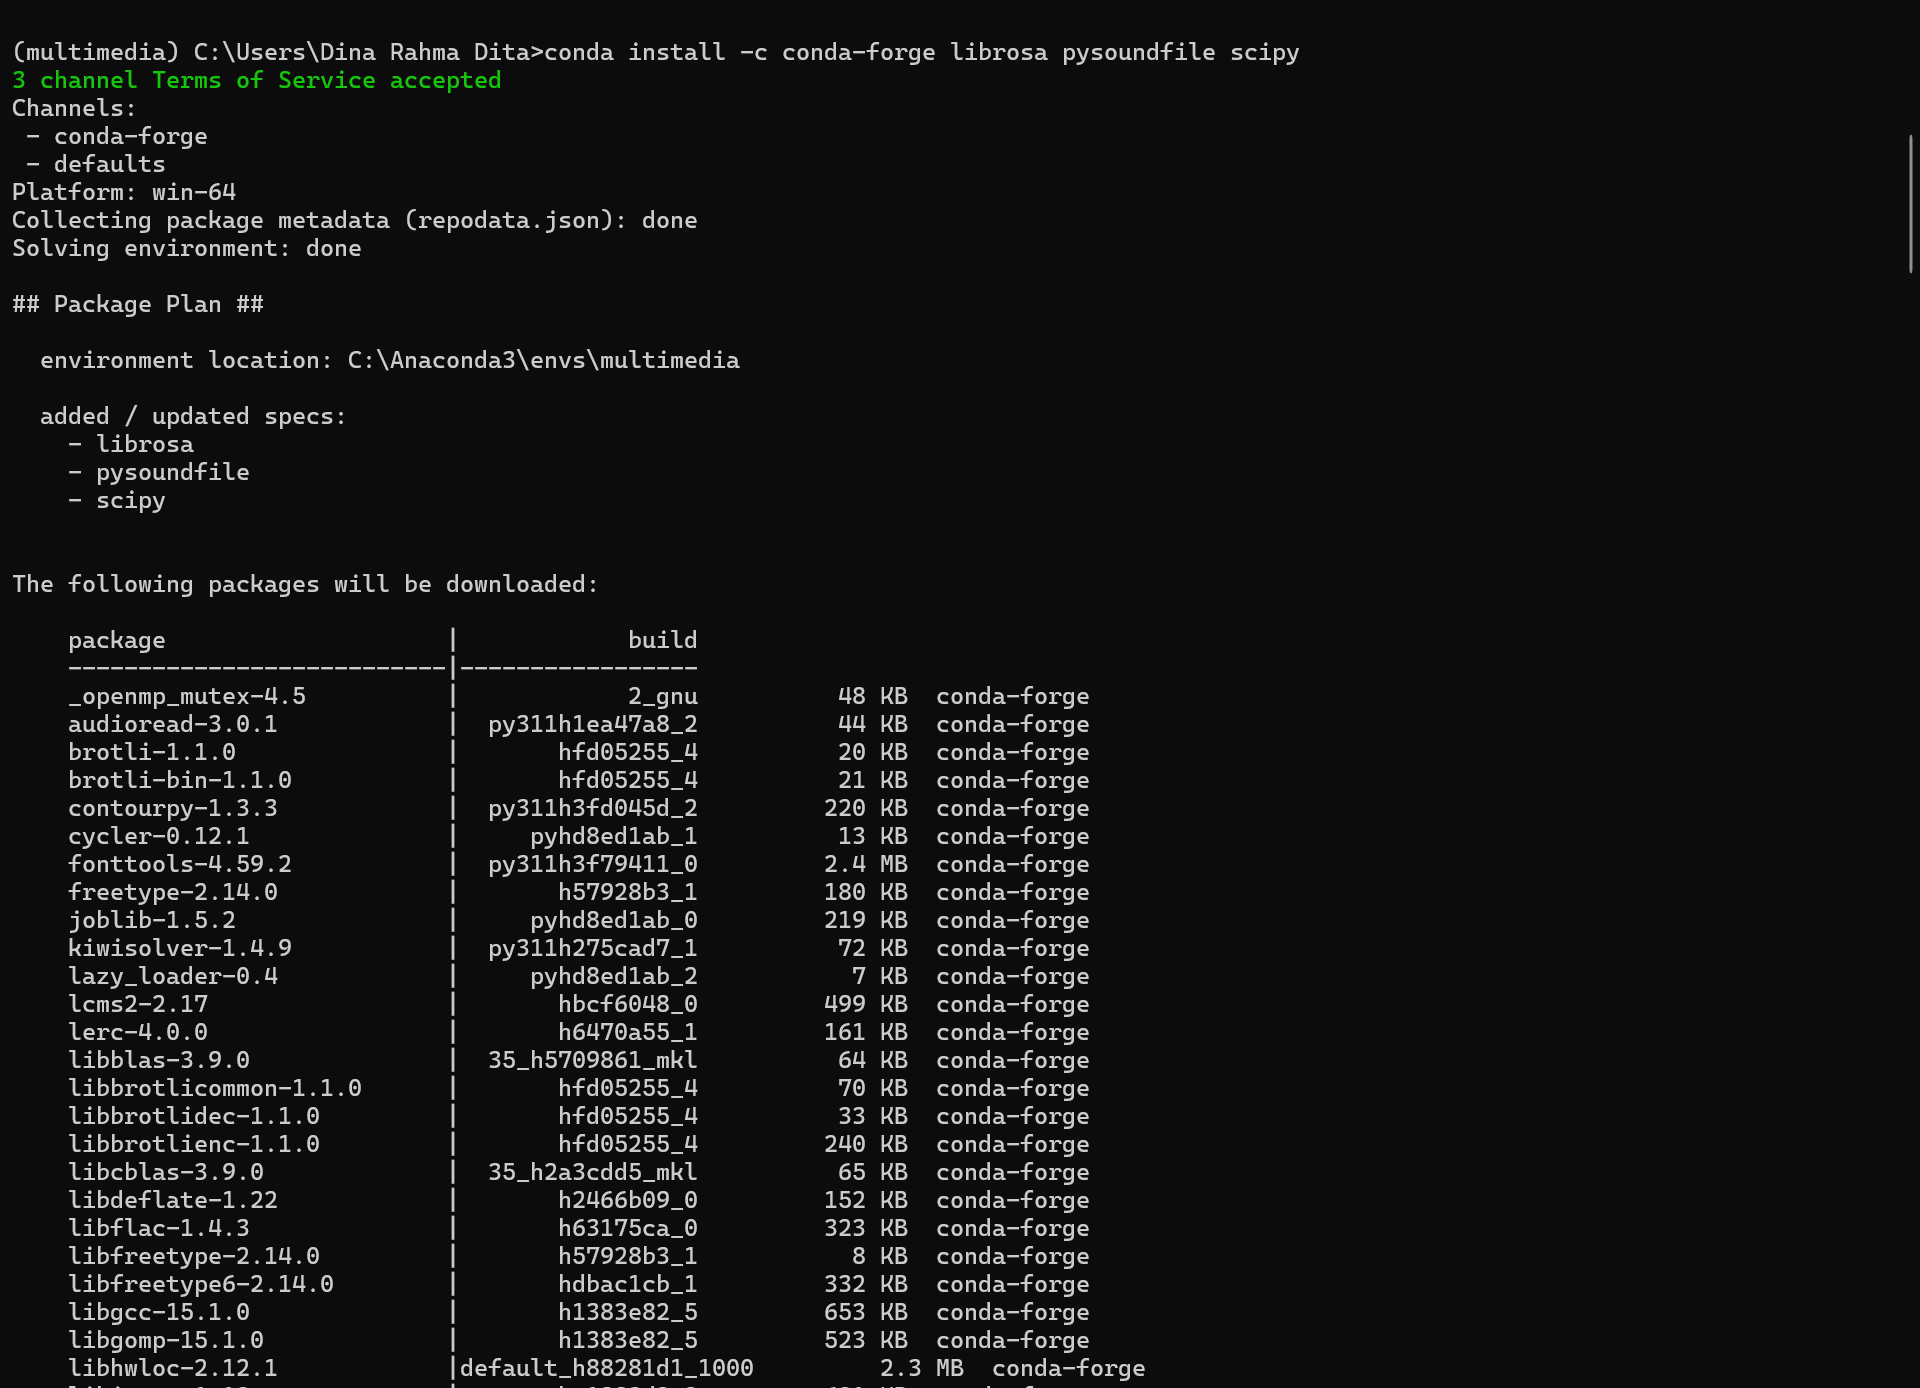
\includegraphics[width=0.7\textwidth]{Figure/ss/3.png}
    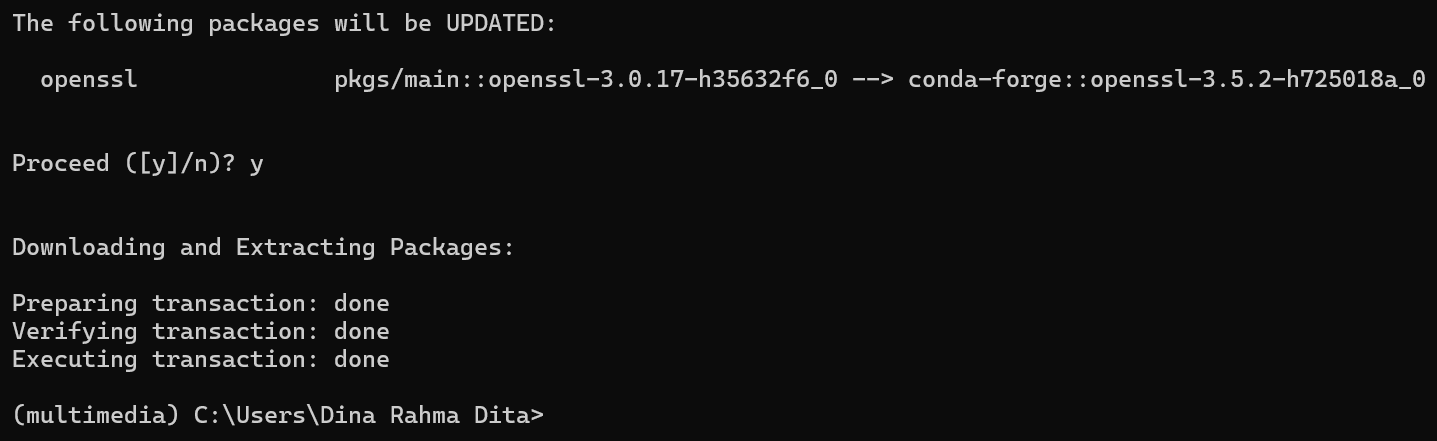
\includegraphics[width=0.7\textwidth]{Figure/ss/4.png}
    \caption{Tampilan proses instalasi library audio di terminal}
    \label{fig:audio_library}
\end{figure}

\subsubsection{Library Image Processing}
\begin{lstlisting}[language=bash, caption=Instalasi library image]
# Untuk conda:
conda install -c conda-forge opencv pillow scikit-image matplotlib
\end{lstlisting}

\begin{figure}[H]
    \centering
    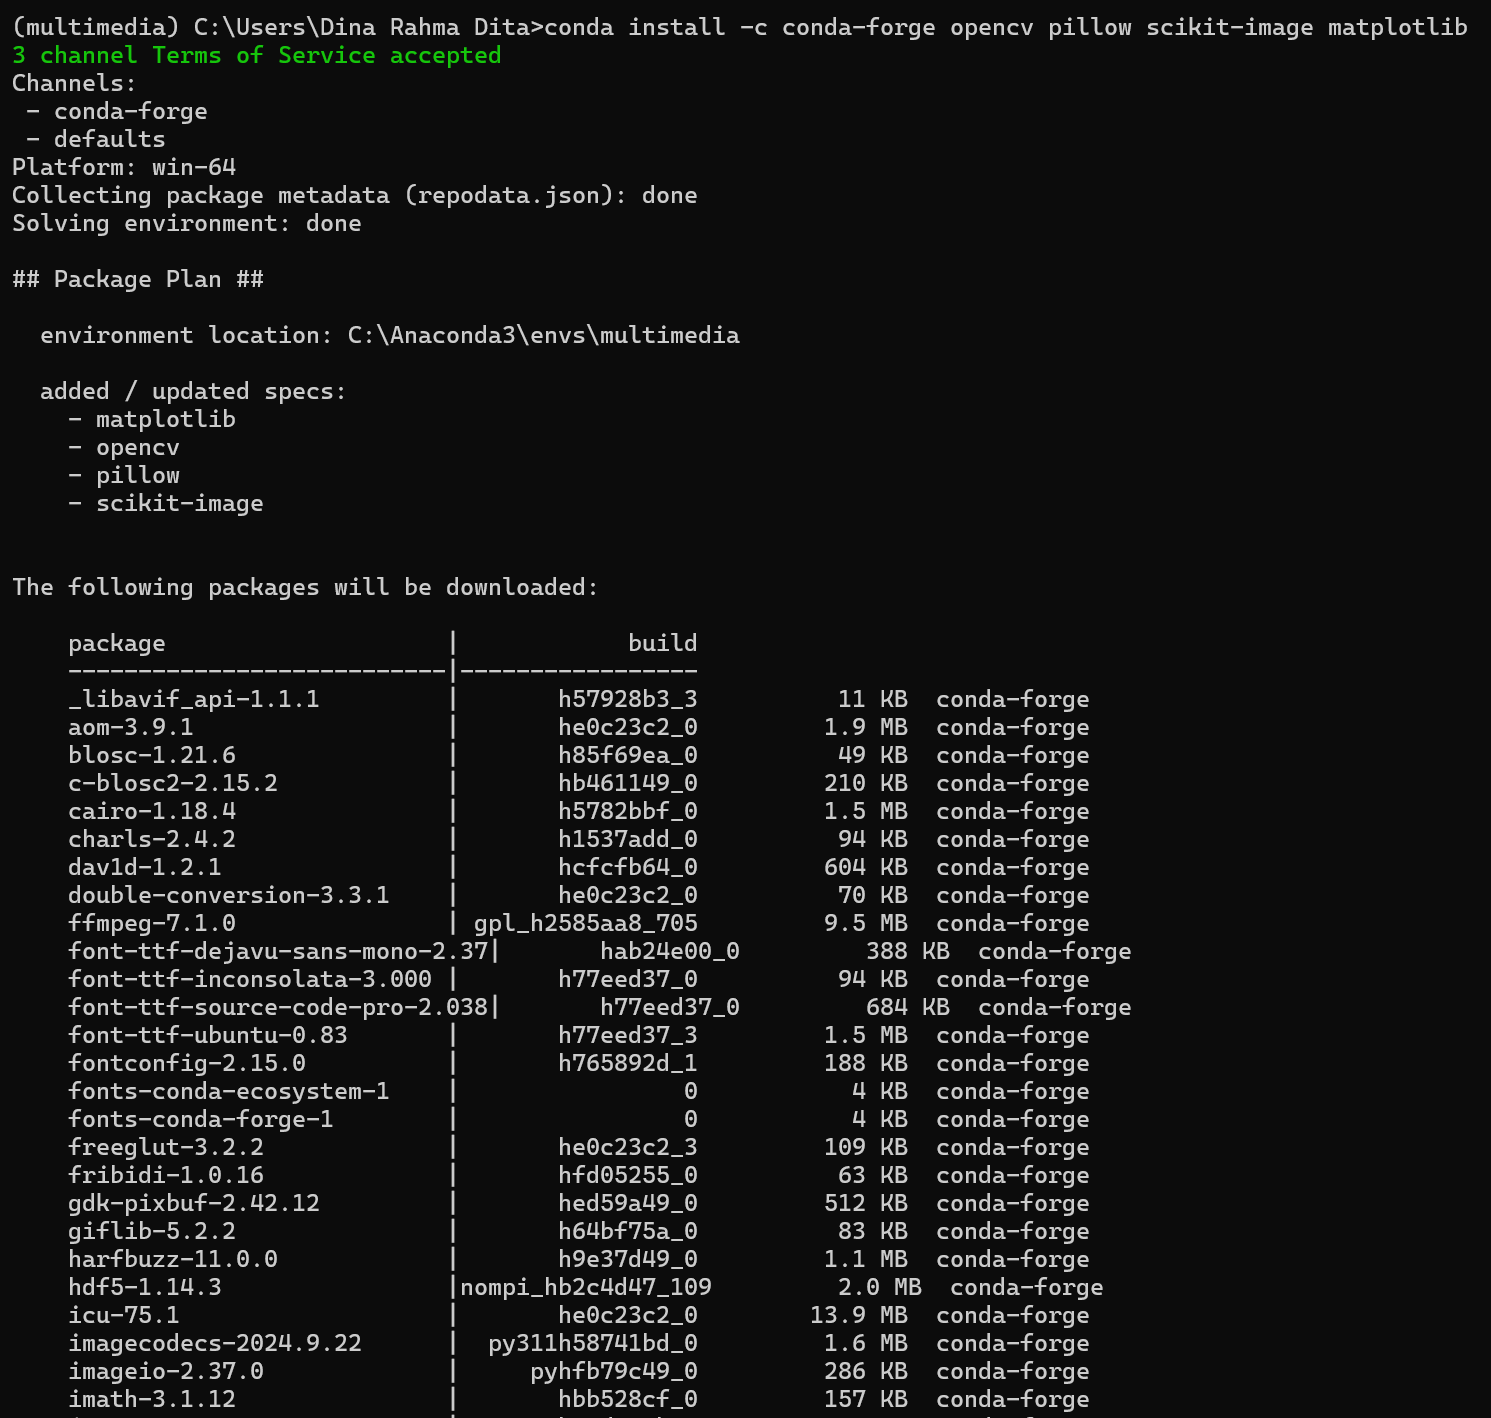
\includegraphics[width=0.7\textwidth]{Figure/ss/5.png}
    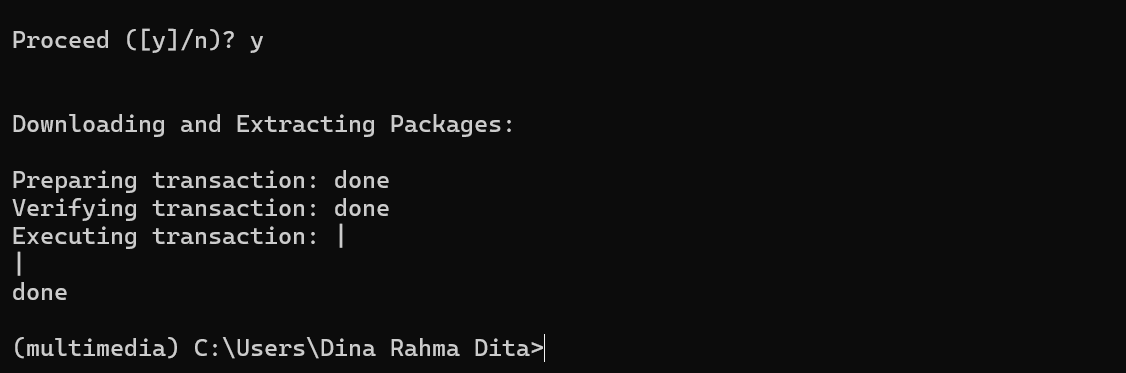
\includegraphics[width=0.7\textwidth]{Figure/ss/6.png}
    \caption{Tampilan proses instalasi library image processing di terminal}
    \label{fig:image_library}
\end{figure}

\subsubsection{Library Video Processing}
\begin{lstlisting}[language=bash, caption=Instalasi library video]
# Untuk conda:
conda install -c conda-forge ffmpeg
pip install moviepy

# Untuk pip (venv/uv):
pip install moviepy
\end{lstlisting}

\begin{figure}[H]
    \centering
    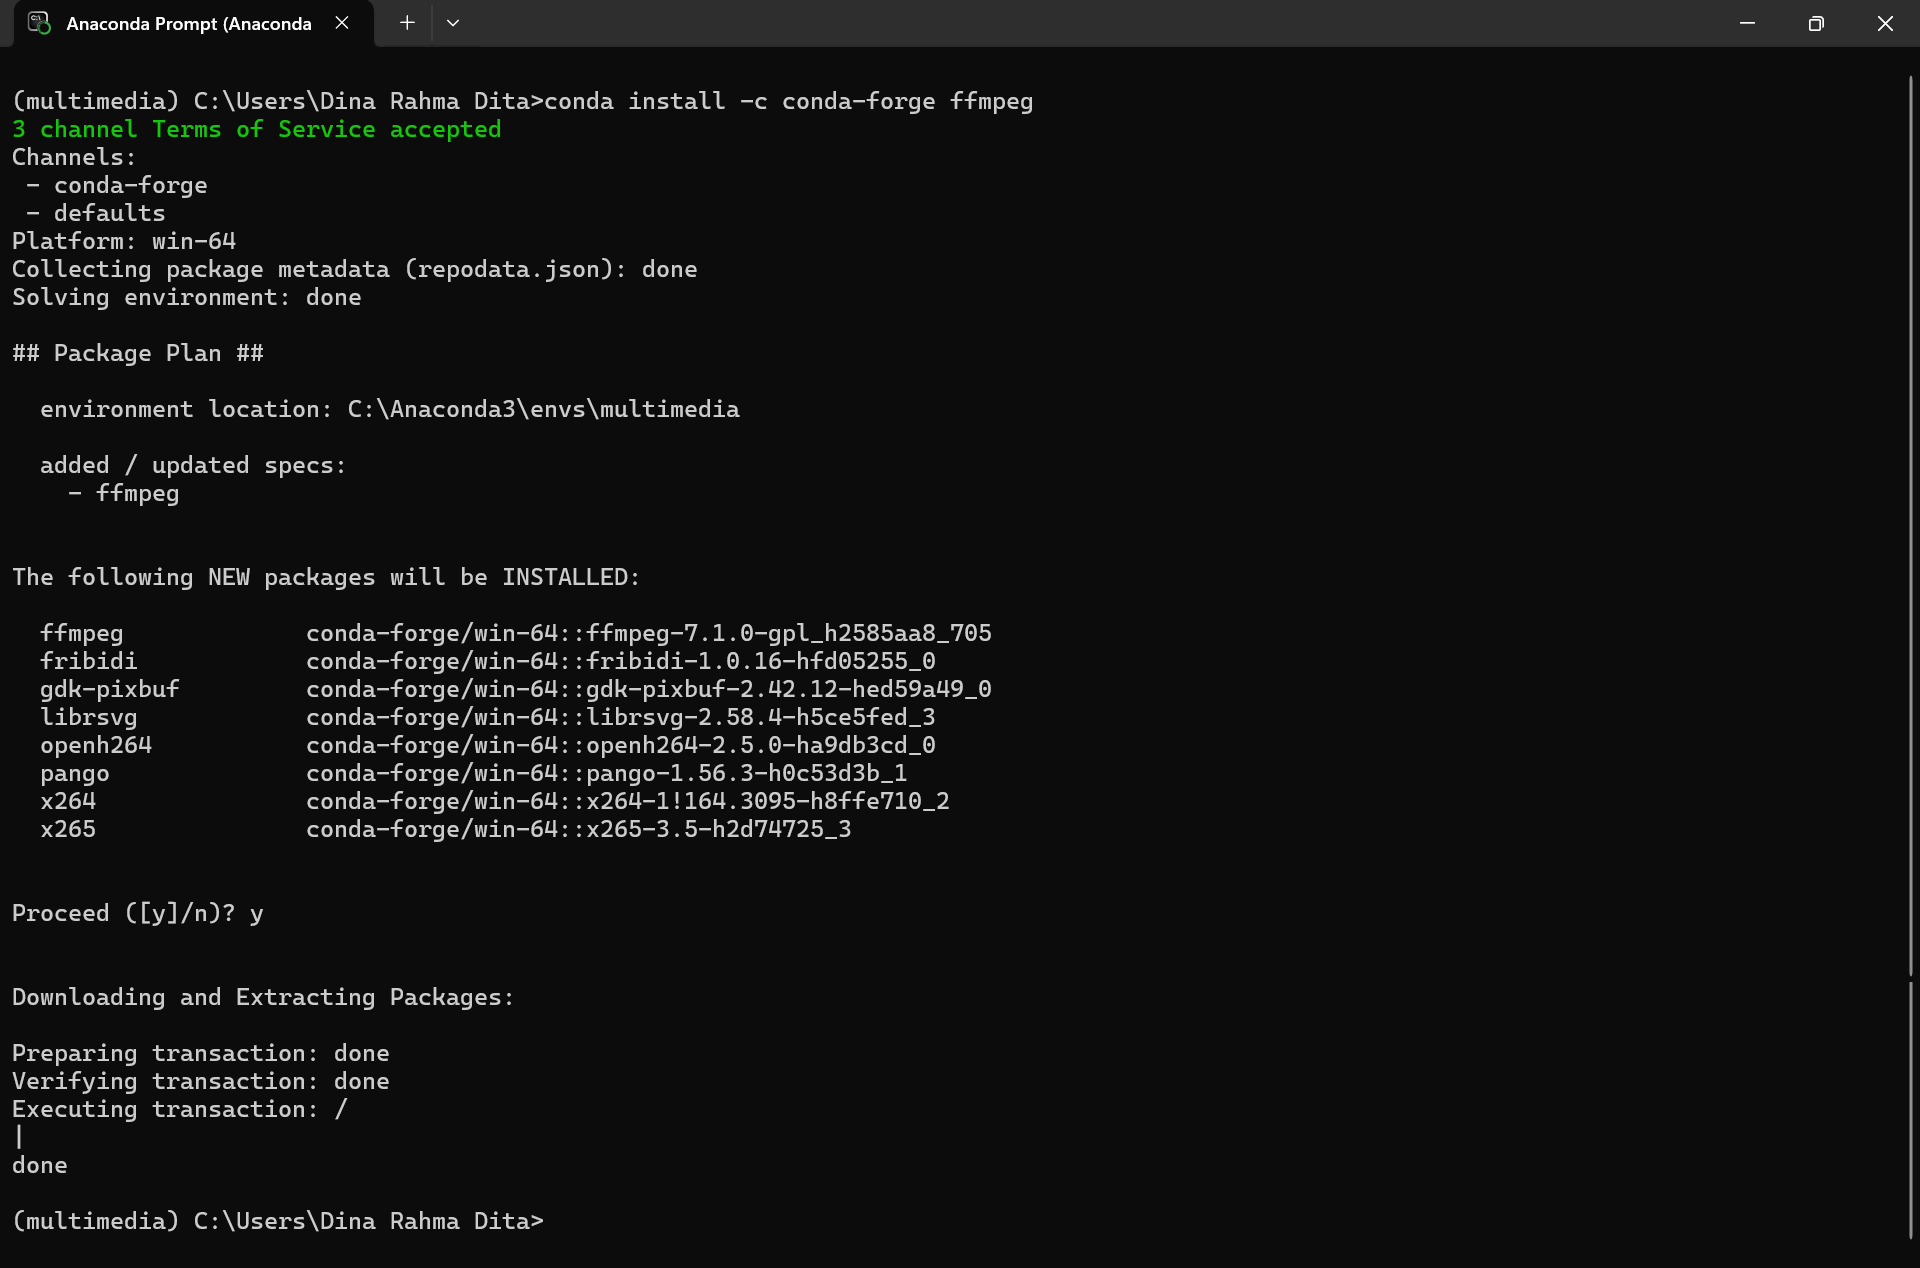
\includegraphics[width=0.7\textwidth]{Figure/ss/7.png}
    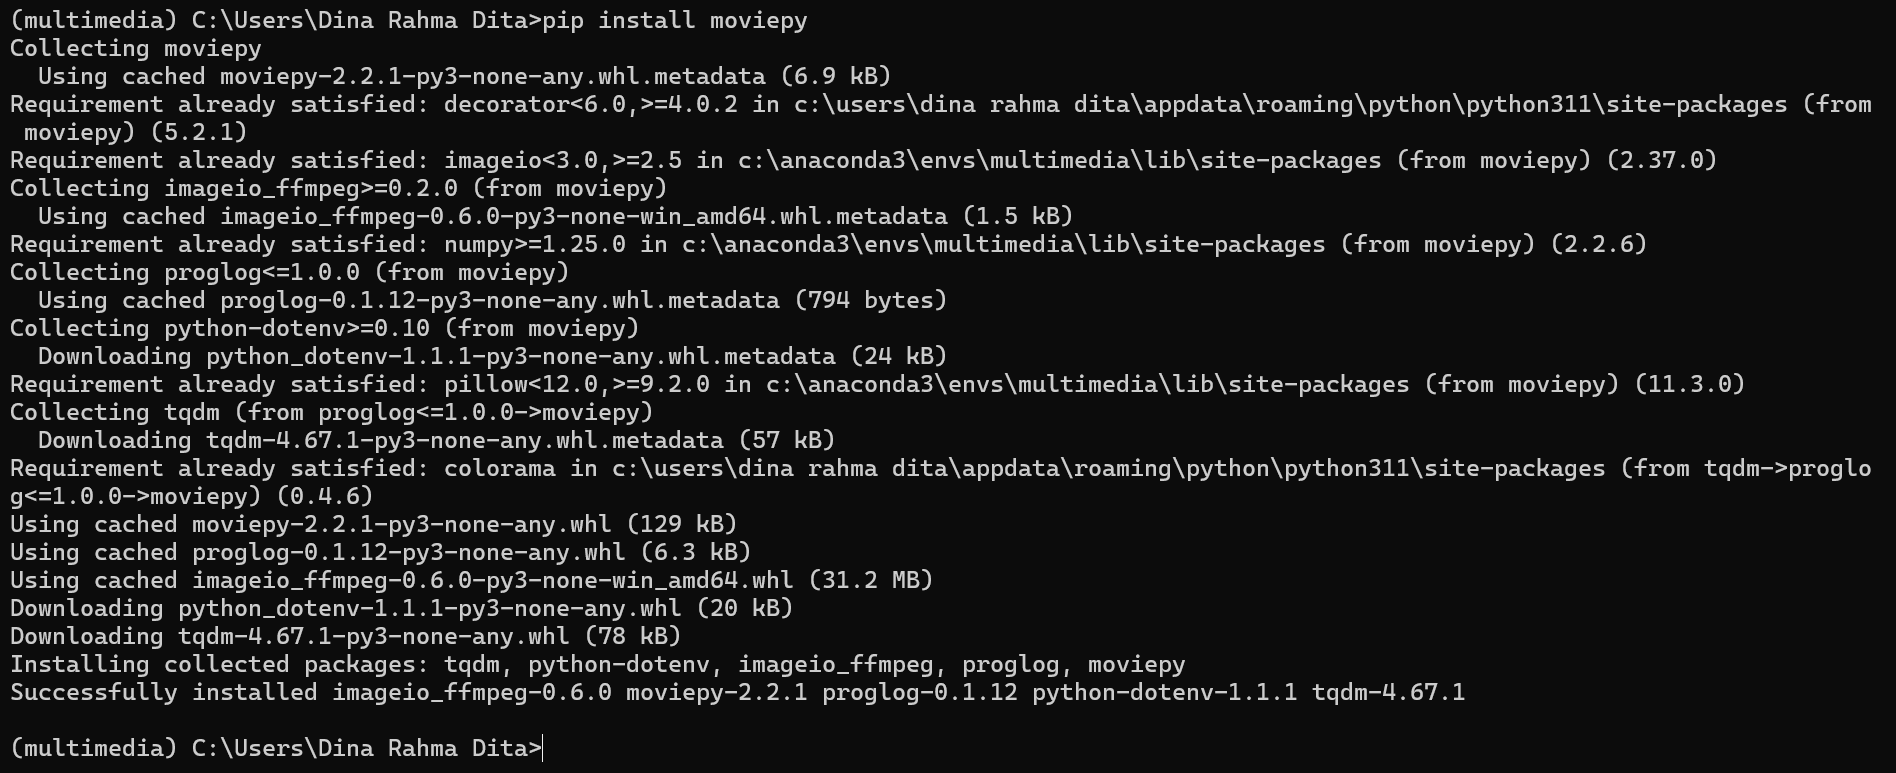
\includegraphics[width=0.7\textwidth]{Figure/ss/8.png}
    \caption{Tampilan proses instalasi library video processing di terminal}
    \label{fig:video_library}
\end{figure}

\subsubsection{Library General Purpose}
\begin{lstlisting}[language=bash, caption=Instalasi library umum]
# Untuk conda:
conda install numpy pandas jupyter

# Untuk pip (venv/uv):
pip install numpy pandas jupyter
\end{lstlisting}

\begin{figure}[H]
    \centering
    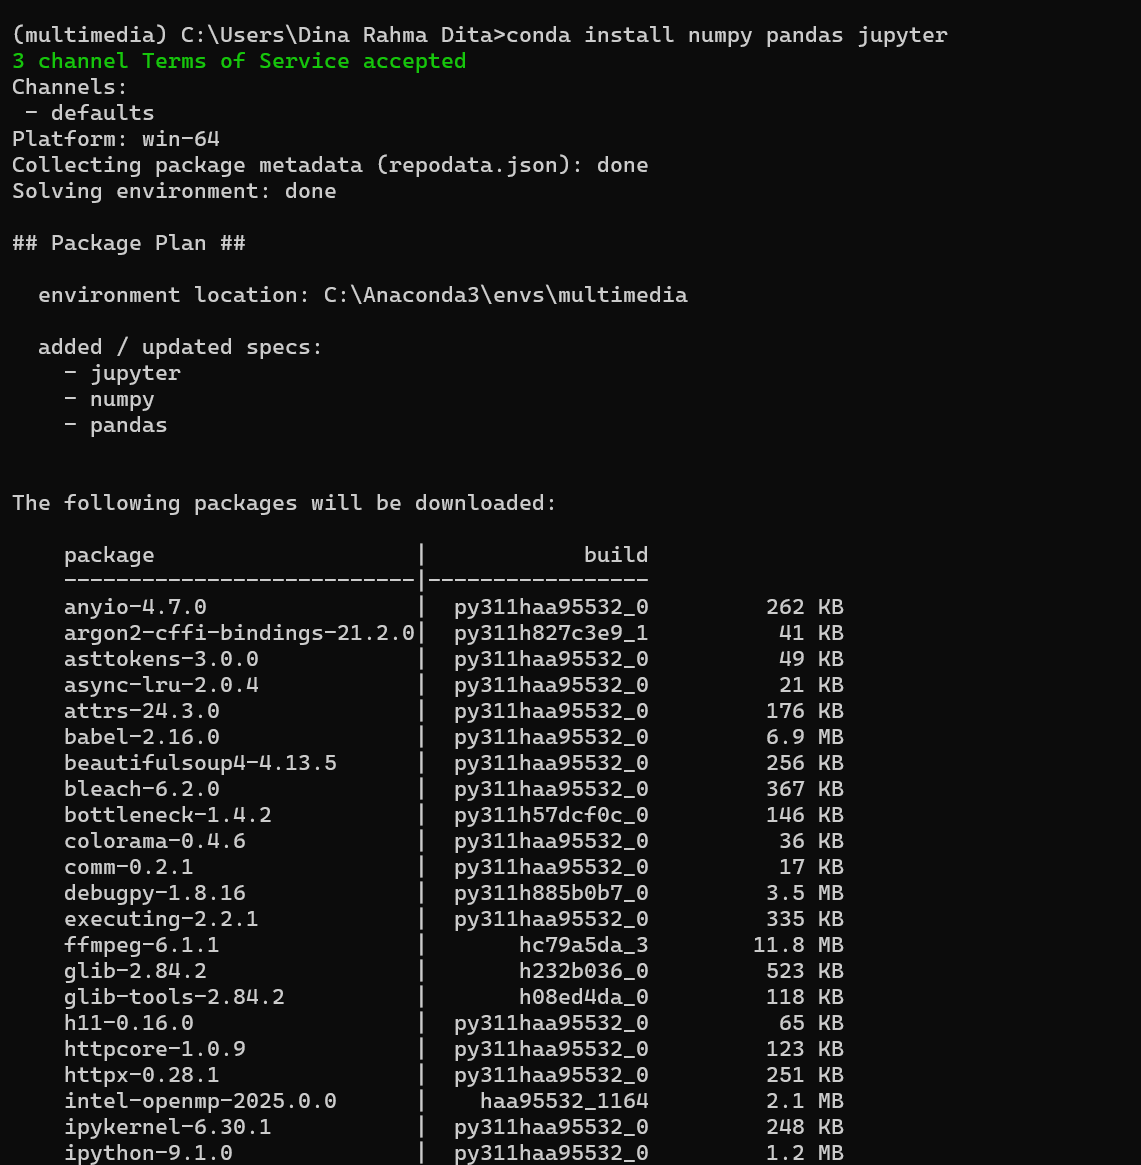
\includegraphics[width=0.7\textwidth]{Figure/ss/9.png}
    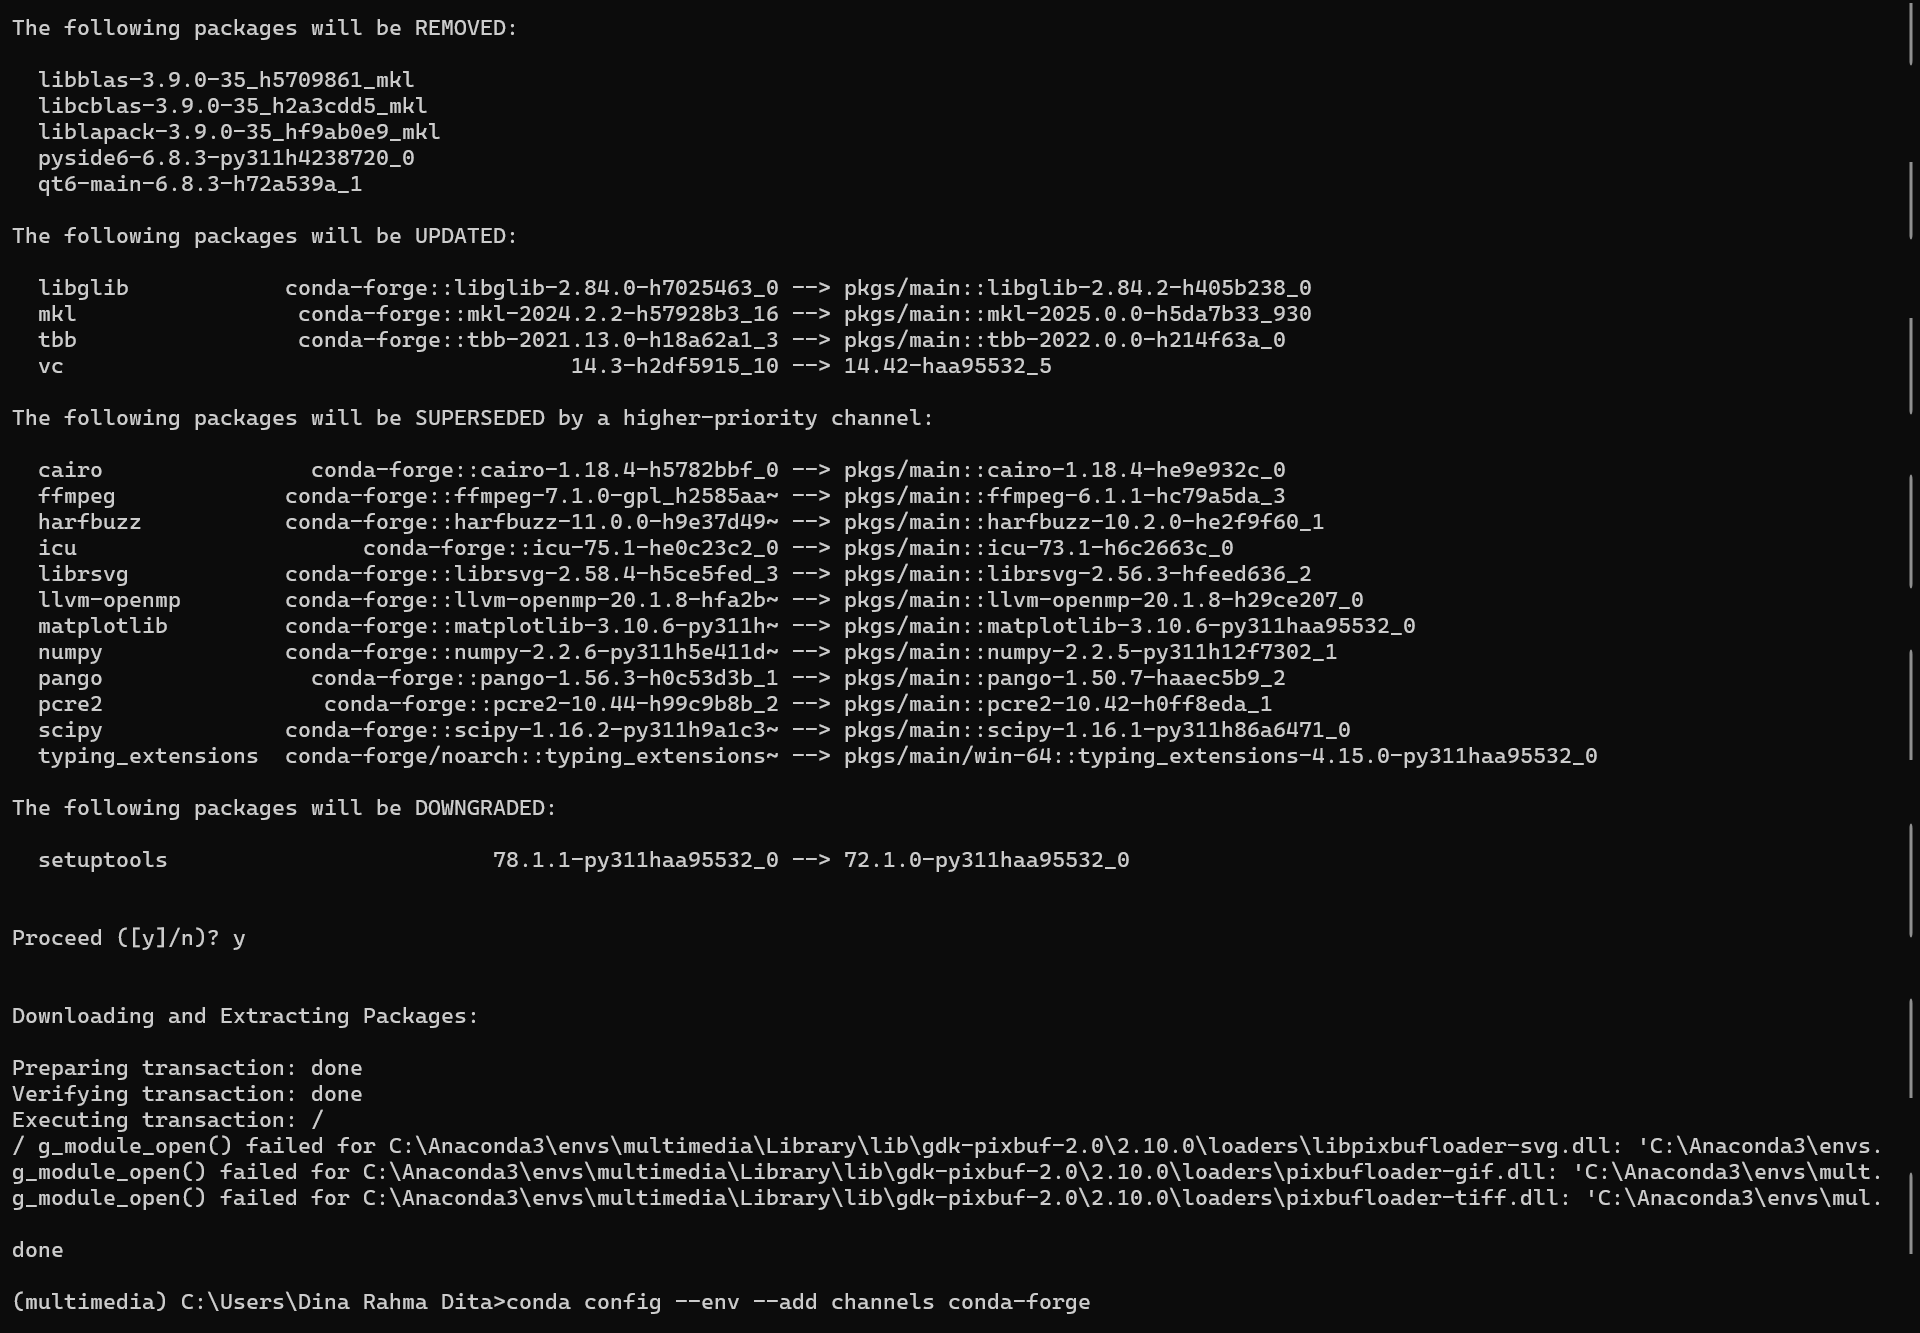
\includegraphics[width=0.7\textwidth]{Figure/ss/10.png}
    \caption{Tampilan proses instalasi library general di terminal}
    \label{fig:library_general}
\end{figure}

\textbf{Dokumentasikan di sini:}
\begin{itemize}
    \item Perintah instalasi yang Anda gunakan
    \item Screenshot proses instalasi atau output sukses
    \item Daftar library yang berhasil diinstall dengan versinya
\end{itemize}

\subsection{Bagian 3: Verifikasi Instalasi}
Buat file Python sederhana untuk menguji semua library yang telah diinstall:

\textbf{Jalankan script dan dokumentasikan hasilnya:}

\begin{figure}[H]
    \centering
    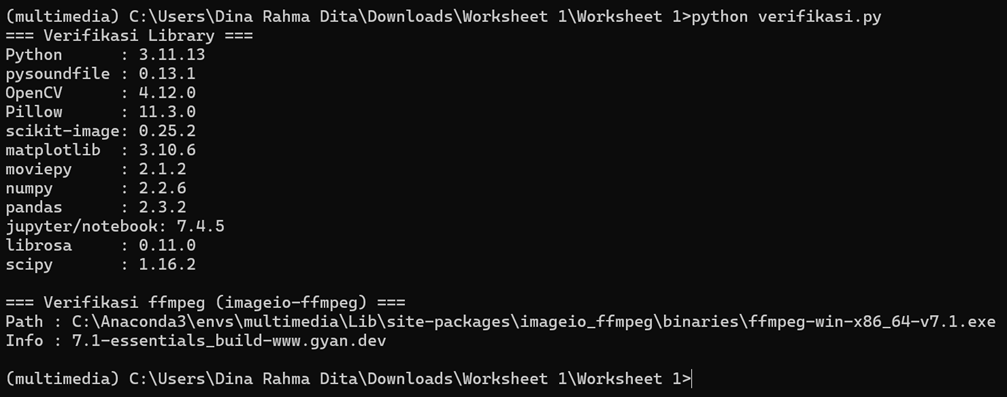
\includegraphics[width=0.7\textwidth]{Figure/ss/11.png}
    \caption{Tampilan hasil verifikasi instalasi library}
    \label{fig:library_verification}
\end{figure}


\subsection{Bagian 4: Simple Test dengan Sample Code}
Buat dan jalankan contoh sederhana untuk setiap kategori multimedia:

\subsubsection{Test Audio Processing}
\begin{lstlisting}[language=Python, caption=Test audio processing sederhana]
import numpy as np
import matplotlib.pyplot as plt

# Generate simple sine wave
duration = 2  # seconds
sample_rate = 44100
frequency = 440  # A4 note

t = np.linspace(0, duration, int(sample_rate * duration))
audio_signal = np.sin(2 * np.pi * frequency * t)

# Plot waveform
plt.figure(figsize=(10, 4))
plt.plot(t[:1000], audio_signal[:1000])  # Plot first 1000 samples
plt.title('Sine Wave (440 Hz)')
plt.xlabel('Time (s)')
plt.ylabel('Amplitude')
plt.grid(True)
plt.savefig('sine_wave_test.png', dpi=150, bbox_inches='tight')
plt.show()

print(f"Generated {duration}s sine wave at {frequency}Hz")
print(f"Sample rate: {sample_rate}Hz")
print(f"Total samples: {len(audio_signal)}")
\end{lstlisting}

\subsubsection{Test Image Processing}
\begin{lstlisting}[language=Python, caption=Test image processing sederhana]
import numpy as np
import matplotlib.pyplot as plt
from PIL import Image

# Create a simple test image
width, height = 400, 300
image = np.zeros((height, width, 3), dtype=np.uint8)

# Add some patterns
image[:, :width//3, 0] = 255  # Red section
image[:, width//3:2*width//3, 1] = 255  # Green section
image[:, 2*width//3:, 2] = 255  # Blue section

# Add a white circle in the center
center_x, center_y = width//2, height//2
radius = 50
Y, X = np.ogrid[:height, :width]
mask = (X - center_x)**2 + (Y - center_y)**2 <= radius**2
image[mask] = [255, 255, 255]

# Display and save
plt.figure(figsize=(8, 6))
plt.imshow(image)
plt.title('Test Image with RGB Stripes and White Circle')
plt.axis('off')
plt.savefig('test_image.png', dpi=150, bbox_inches='tight')
plt.show()

print(f"Created test image: {width}x{height} pixels")
print(f"Image shape: {image.shape}")
print(f"Image dtype: {image.dtype}")
\end{lstlisting}

\textbf{Dokumentasikan hasil eksekusi:}
\begin{itemize}
    \item Screenshot output dari kedua script di atas
    \item Gambar yang dihasilkan (sine\_wave\_test.png dan test\_image.png)
    \item Error message jika ada dan cara mengatasinya
\end{itemize}

\subsubsection{Test Audio Processing}
\begin{figure}[H]
    \centering
    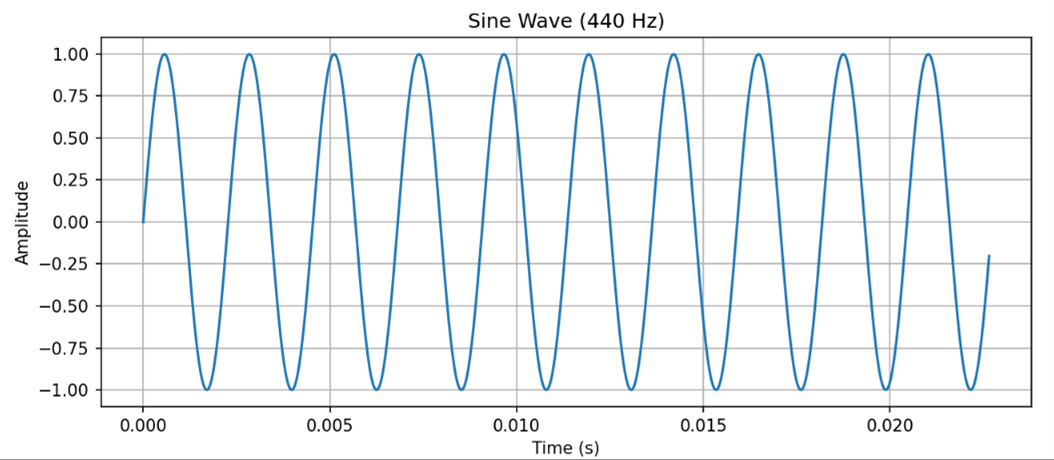
\includegraphics[width=0.7\textwidth]{Figure/ss/12.png}
    \caption{Tampilan hasil test audio processing}
    \label{fig:audio_processing}
\end{figure}

\subsubsection{Test Image Processing}
\begin{figure}[H]
    \centering
    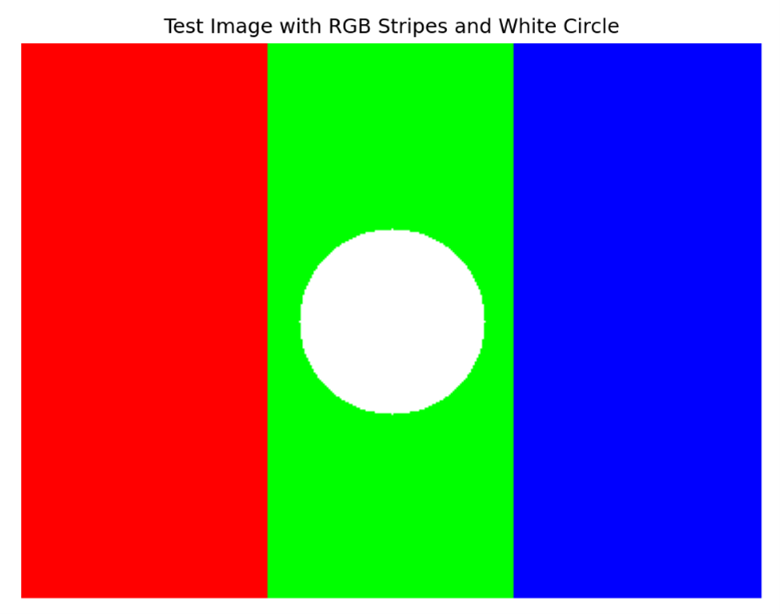
\includegraphics[width=0.7\textwidth]{Figure/ss/13.png}
    \caption{Tampilan hasil test image processing}
    \label{fig:image_processing}
\end{figure}

\section{Bagian Laporan}

\subsection{Output Verifikasi Instalasi}
\textbf{Copy-paste output lengkap dari script \texttt{test\_multimedia.py} di sini:}

\begin{figure}[H]
    \centering
    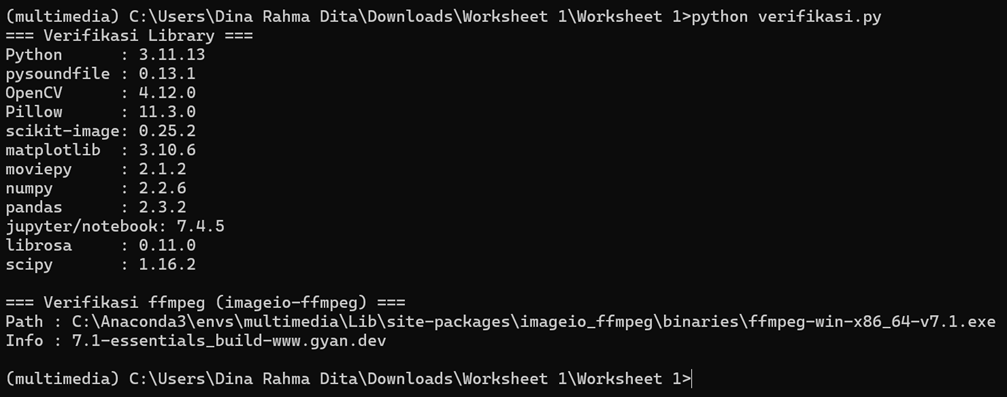
\includegraphics[width=0.7\textwidth]{Figure/ss/11.png}
    \caption{Output verifikasi instalasi library}
    \label{fig:verifikasi_library}
\end{figure}

\subsection{Screenshot Hasil Test}
\textbf{Sisipkan screenshot atau gambar hasil dari:}
\begin{itemize}
    \item Terminal/command prompt yang menunjukkan environment aktif
    \begin{figure}[H]
        \centering
        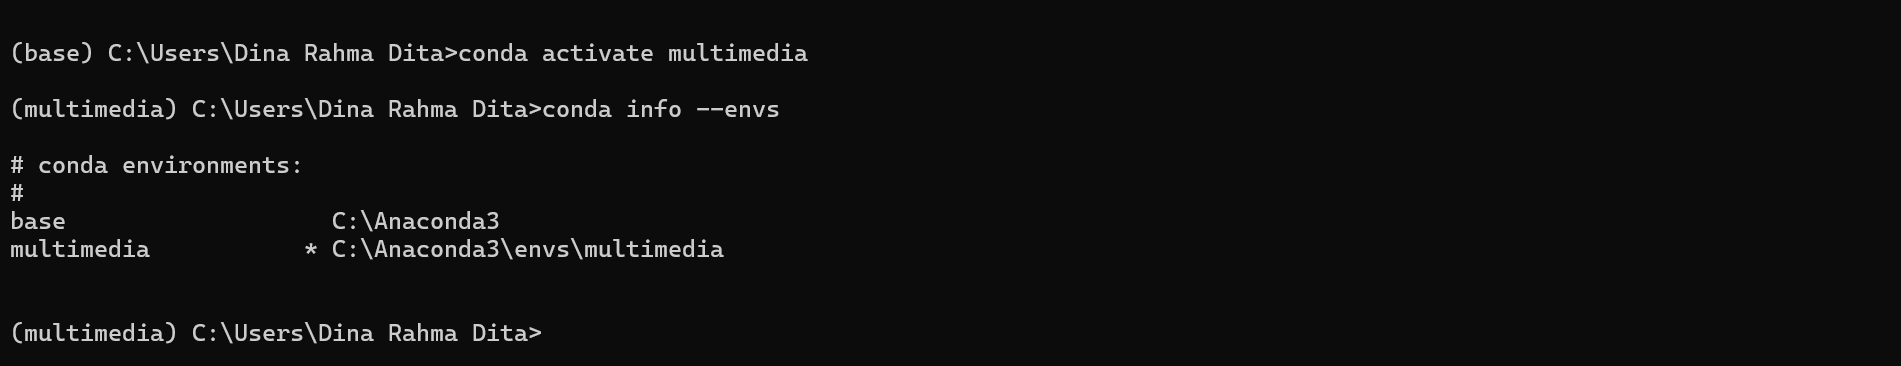
\includegraphics[width=0.7\textwidth]{Figure/ss/2.png}
    \caption{Tampilan environment aktif di terminal}
    \label{fig:env_terminal}
    \end{figure}

    \item Output dari script test audio (sine wave plot)
    \begin{figure}[H]
        \centering
        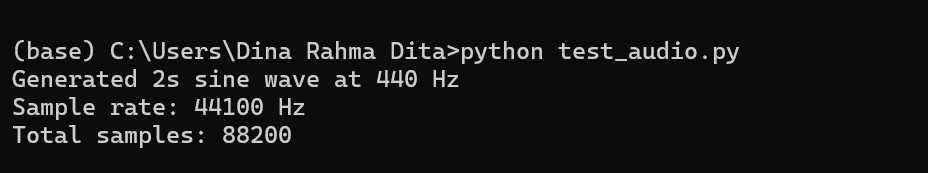
\includegraphics[width=0.7\textwidth]{Figure/ss/14.png}
        \caption{Output sine wave plot dari test audio processing}
        \label{fig:audio_sine_wave}
    \end{figure}

    \item Output dari script test image (RGB stripes dengan circle)
    \begin{figure}[H]
        \centering
        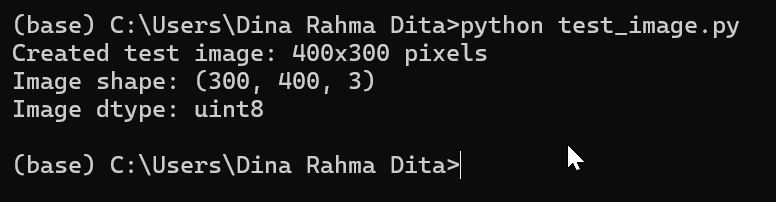
\includegraphics[width=0.7\textwidth]{Figure/ss/15.png}
    \caption{Output RGB stripes dengan circle dari test image processing}
    \label{fig:image_rgb}
    \end{figure}
\end{itemize}

\textit{Gunakan perintah \textbackslash\texttt{includegraphics} untuk menyisipkan gambar}

\subsection{Analisis dan Refleksi}
\textbf{Jawab pertanyaan berikut:}

\begin{enumerate}
    \item \textbf{Mengapa penting menggunakan environment terpisah untuk project multimedia?}
    
    \textit{[Dalam mengerjakan project multimedia biasanya  memakai banyak software dengan versi yang berbeda, bahkan kadang lintas sistem operasi jika dikerjakan bersama tim. Supaya project tidak rusak atau bermasalah, penting untuk membuat sebuah environment. Dengan adanya environment yang sama, semua kebutuhan sudah diseragamkan sehingga project bisa lebih stabil dan aman untuk dikerjakan bersama dengan tim.]}
    
    \item \textbf{Apa perbedaan utama antara conda, venv, dan uv? Mengapa Anda memilih tool yang Anda gunakan?}
    
    \textit{[Perbedaan antara conda, venv dan uv : \\
Conda = Bisa digunakan untuk library eksternal selain python, bahkan lintas bahasa lumayan powerfull  tapi cukup berat dijalankan. Cocok untuk project ringan \\
Venv = Digunakan untuk library pure python, tidak bisa untuk library eksternal non-python \\
Uv = Dapat menginstall package python dengan lebih tapi uv belum sekomplit conda
]}
    
    \item \textbf{Library mana yang paling sulit diinstall dan mengapa?}
    
    \textit{[Tidak terlalu sulit untuk menginstall library yang diminta, hanya ada sedikit masalah seperti pada saat menginstall library audio, ternyata dalam penulisannya harus ditulis pysoundfile bukan soundfile dan  beda soundfile dan pysoundfile itu adalah jika soundfile itu modulnya maka pysoundfile itu librarynya.]}
    
    \item \textbf{Bagaimana cara mengatasi masalah dependency conflict jika terjadi?}
    
    \textit{[Ada beberapa cara untuk mengatasi dependency conflict berdasarkan yang sudah saya lakukan : \\
-	Untuk mencegah konflik dengan projek lain maka dibuatlah environment terpisah (multimedia)\\
-	Melakukan downgrade atau upgrade agar tetap kompatibel, gunakan satu channel saja seperti conda-forge pada saat proses penginstallan untuk menghindari konflik dan file rusak. \\
-	Mengatur channel priority supaya library atau paket yang di install sumbernya hanya dari conda-forge \\
-	Jika konflik sudah terlalu berat maka bahkanuat ulang environment dan install ulang library yang dibutuhkan
]}
    
    \item \textbf{Jelaskan fungsi dari masing-masing library yang berhasil Anda install!}
    
    \begin{itshape}
    librosa = analisis \& ekstraksi fitur audio (MFCC, spectrogram). \par
    scipy = fungsi matematis \& scientific (filter, transformasi). \par
    pysoundfile = baca/tulis file audio (WAV, FLAC, OGG). \par
    OpenCV (cv2) = olah gambar \& video (deteksi objek, transformasi). \par
    Pillow (PIL) = manipulasi gambar sederhana (resize, crop, ubah format). \par
    scikit-image = image processing scientific (segmentasi, edge detection). \par
    matplotlib = visualisasi data/grafik, tampilkan gambar \& waveform audio. \par
    ffmpeg = backend encoding/decoding audio-video. \par
    moviepy = editing video (cut, merge, tambah teks/suara). \par
    numpy = komputasi numerik \& array multidimensi. \par
    pandas = olah data tabular/metadata multimedia. \par
    jupyter/notebook = coding interaktif, dokumentasi, \& visualisasi.
    \end{itshape}
\end{enumerate}

\subsection{Troubleshooting}
\textbf{Dokumentasikan masalah yang Anda hadapi (jika ada) dan cara mengatasinya:}

\begin{itemize}
    \item \textbf{Masalah 1:} \textit{[Terkendala saat proses menginstall library audio karena tidak bisa menemukan modul soundfile]}
    
    \textbf{Solusi:} \textit{[mengganti ke pysoundfile bukan soundfile pada saat proses instalasi library audio]}
    
\end{itemize}

\section{Export Environment untuk Reproduksi}
Sebagai langkah terakhir, export environment Anda agar dapat direproduksi:

\subsection{Untuk Conda}
\begin{lstlisting}[language=bash, caption=Export conda environment]
conda env export > environment.yml
\end{lstlisting}

\subsection{Untuk venv/uv}
\begin{lstlisting}[language=bash, caption=Export pip requirements]
pip freeze > requirements.txt
\end{lstlisting}

\textbf{Copy-paste isi file environment.yml atau requirements.txt di sini:}

\begin{lstlisting}[caption=Environment/Requirements file]
[name: multimedia
channels:
  - conda-forge
  - defaults
dependencies:
  - _libavif_api=1.1.1=h57928b3_3
  - _openmp_mutex=4.5=2_gnu
  - anyio=4.7.0=py311haa95532_0
  - aom=3.9.1=he0c23c2_0
  - argon2-cffi=21.3.0=pyhd3eb1b0_0
  - argon2-cffi-bindings=21.2.0=py311h827c3e9_1
  - asttokens=3.0.0=py311haa95532_0
  - async-lru=2.0.4=py311haa95532_0
  - attrs=24.3.0=py311haa95532_0
  - audioread=3.0.1=py311h1ea47a8_2
  - babel=2.16.0=py311haa95532_0
  - beautifulsoup4=4.13.5=py311haa95532_0
  - blas=1.0=mkl
  - bleach=6.2.0=py311haa95532_0
  - blosc=1.21.6=h85f69ea_0
  - bottleneck=1.4.2=py311h57dcf0c_0
  - brotli=1.1.0=hfd05255_4
  - brotli-bin=1.1.0=hfd05255_4
  - brotli-python=1.1.0=py311h3e6a449_4
  - bzip2=1.0.8=h2bbff1b_6
  - c-blosc2=2.15.2=hb461149_0
  - ca-certificates=2025.9.9=haa95532_0
  - cairo=1.18.0=h91e5215_2
  - certifi=2025.8.3=pyhd8ed1ab_0
  - cffi=1.17.1=py311h3485c13_1
  - charls=2.4.2=h1537add_0
  - charset-normalizer=3.4.3=pyhd8ed1ab_0
  - colorama=0.4.6=py311haa95532_0
  - comm=0.2.1=py311haa95532_0
  - contourpy=1.3.3=py311h3fd045d_2
  - cycler=0.12.1=pyhd8ed1ab_1
  - dav1d=1.2.1=hcfcfb64_0
  - debugpy=1.8.16=py311h885b0b7_0
  - decorator=5.2.1=pyhd8ed1ab_0
  - defusedxml=0.7.1=pyhd3eb1b0_0
  - double-conversion=3.3.1=he0c23c2_0
  - executing=2.2.1=py311haa95532_0
  - expat=2.7.1=h8ddb27b_0
  - ffmpeg=6.1.1=hc79a5da_3
  - font-ttf-dejavu-sans-mono=2.37=hab24e00_0
  - font-ttf-inconsolata=3.000=h77eed37_0
  - font-ttf-source-code-pro=2.038=h77eed37_0
  - font-ttf-ubuntu=0.83=h77eed37_3
  - fontconfig=2.15.0=h765892d_1
  - fonts-conda-ecosystem=1=0
  - fonts-conda-forge=1=0
  - fonttools=4.59.2=py311h3f79411_0
  - freeglut=3.2.2=he0c23c2_3
  - freetype=2.14.0=h57928b3_1
  - fribidi=1.0.16=hfd05255_0
  - gdk-pixbuf=2.42.12=hed59a49_0
  - giflib=5.2.2=h64bf75a_0
  - glib=2.80.2=h0df6a38_0
  - glib-tools=2.80.2=h2f9d560_0
  - graphite2=1.3.14=hac47afa_2
  - h11=0.16.0=py311haa95532_0
  - h2=4.3.0=pyhcf101f3_0
  - harfbuzz=10.2.0=he2f9f60_1
  - hdf5=1.14.3=nompi_hb2c4d47_109
  - hpack=4.1.0=pyhd8ed1ab_0
  - httpcore=1.0.9=py311haa95532_0
  - httpx=0.28.1=py311haa95532_0
  - hyperframe=6.1.0=pyhd8ed1ab_0
  - icc_rt=2022.1.0=h6049295_2
  - icu=73.2=h63175ca_0
  - idna=3.10=pyhd8ed1ab_1
  - imagecodecs=2024.9.22=py311h58741bd_0
  - imageio=2.37.0=pyhfb79c49_0
  - imath=3.1.12=hbb528cf_0
  - importlib-metadata=8.7.0=pyhe01879c_1
  - intel-openmp=2024.2.1=h57928b3_1083
  - ipykernel=6.30.1=py311haa95532_0
  - ipython=9.1.0=py311haa95532_0
  - ipython_pygments_lexers=1.1.1=py311haa95532_0
  - ipywidgets=8.1.5=py311haa95532_0
  - jasper=4.2.8=h8ad263b_0
  - jedi=0.19.2=py311haa95532_0
  - jinja2=3.1.6=py311haa95532_0
  - joblib=1.5.2=pyhd8ed1ab_0
  - json5=0.9.25=py311haa95532_0
  - jsonschema=4.25.0=py311haa95532_0
  - jsonschema-specifications=2023.7.1=py311haa95532_0
  - jupyter=1.1.1=py311haa95532_0
  - jupyter-lsp=2.2.5=py311haa95532_0
  - jupyter_client=8.6.3=py311haa95532_0
  - jupyter_console=6.6.3=py311haa95532_0
  - jupyter_core=5.8.1=py311haa95532_0
  - jupyter_events=0.12.0=py311haa95532_0
  - jupyter_server=2.16.0=py311haa95532_0
  - jupyter_server_terminals=0.5.3=py311haa95532_0
  - jupyterlab=4.4.6=py311haa95532_0
  - jupyterlab_pygments=0.3.0=py311haa95532_0
  - jupyterlab_server=2.27.3=py311haa95532_0
  - jupyterlab_widgets=3.0.15=py311haa95532_0
  - jxrlib=1.1=hcfcfb64_3
  - khronos-opencl-icd-loader=2024.10.24=h2466b09_1
  - kiwisolver=1.4.9=py311h275cad7_1
  - krb5=1.21.3=hdf4eb48_0
  - lame=3.100=hcfcfb64_1003
  - lazy-loader=0.4=pyhd8ed1ab_2
  - lazy_loader=0.4=pyhd8ed1ab_2
  - lcms2=2.17=hbcf6048_0
  - lerc=4.0.0=h6470a55_1
  - libabseil=20240116.2=cxx17_he0c23c2_1
  - libaec=1.1.4=h20038f6_0
  - libasprintf=0.22.5=h5728263_3
  - libavif16=1.1.1=h4d049a7_2
  - libblas=3.9.0=26_win64_mkl
  - libbrotlicommon=1.1.0=hfd05255_4
  - libbrotlidec=1.1.0=hfd05255_4
  - libbrotlienc=1.1.0=hfd05255_4
  - libcblas=3.9.0=26_win64_mkl
  - libclang13=21.1.1=default_ha2db4b5_0
  - libcurl=8.14.1=h88aaa65_0
  - libdeflate=1.22=h2466b09_0
  - libexpat=2.7.1=hac47afa_0
  - libffi=3.4.4=hd77b12b_1
  - libflac=1.4.3=h63175ca_0
  - libfreetype=2.14.0=h57928b3_1
  - libfreetype6=2.14.0=hdbac1cb_1
  - libgcc=15.1.0=h1383e82_5
  - libgettextpo=0.22.5=h5728263_3
  - libglib=2.80.2=h0df6a38_0
  - libgomp=15.1.0=h1383e82_5
  - libhwloc=2.12.1=default_h88281d1_1000
  - libhwy=1.3.0=h47aaa27_0
  - libiconv=1.18=hc1393d2_2
  - libintl=0.22.5=h5728263_3
  - libintl-devel=0.22.5=h5728263_3
  - libjpeg-turbo=3.1.0=h2466b09_0
  - libjxl=0.11.1=hb7713f0_4
  - liblapack=3.9.0=26_win64_mkl
  - liblapacke=3.9.0=26_win64_mkl
  - libogg=1.3.5=h2466b09_1
  - libopenvino=2024.2.0=hfe1841e_1
  - libopenvino-auto-batch-plugin=2024.2.0=h04f32e0_1
  - libopenvino-auto-plugin=2024.2.0=h04f32e0_1
  - libopenvino-hetero-plugin=2024.2.0=h372dad0_1
  - libopenvino-intel-cpu-plugin=2024.2.0=hfe1841e_1
  - libopenvino-intel-gpu-plugin=2024.2.0=hfe1841e_1
  - libopenvino-ir-frontend=2024.2.0=h372dad0_1
  - libopenvino-onnx-frontend=2024.2.0=hdeef14f_1
  - libopenvino-paddle-frontend=2024.2.0=hdeef14f_1
  - libopenvino-pytorch-frontend=2024.2.0=he0c23c2_1
  - libopenvino-tensorflow-frontend=2024.2.0=h7c40eac_1
  - libopenvino-tensorflow-lite-frontend=2024.2.0=he0c23c2_1
  - libopus=1.5.2=h2466b09_0
  - libpng=1.6.50=h7351971_1
  - libpq=12.15=h906ac69_0
  - libprotobuf=4.25.3=h47a098d_1
  - librosa=0.11.0=pyhd8ed1ab_0
  - librsvg=2.56.3=hfeed636_2
  - libsndfile=1.2.2=h81429f1_1
  - libsodium=1.0.20=h83e8143_0
  - libsqlite=3.50.4=hf5d6505_0
  - libssh2=1.11.1=h9aa295b_0
  - libtheora=1.1.1=h8cc25b3_3
  - libtiff=4.7.0=hfc51747_1
  - libvorbis=1.3.7=h5112557_2
  - libwebp-base=1.6.0=h4d5522a_0
  - libwinpthread=12.0.0.r4.gg4f2fc60ca=h57928b3_9
  - libxcb=1.17.0=h0e4246c_0
  - libxml2=2.13.8=h741aa76_1
  - libxslt=1.1.43=h25c3957_0
  - libzlib=1.3.1=h02ab6af_0
  - libzopfli=1.0.3=h0e60522_0
  - llvm-openmp=20.1.8=h29ce207_0
  - llvmlite=0.44.0=py311h7c248df_2
  - lz4-c=1.9.4=hcfcfb64_0
  - markupsafe=3.0.2=py311h827c3e9_0
  - matplotlib=3.10.6=py311haa95532_0
  - matplotlib-base=3.10.6=py311h1675fdf_1
  - matplotlib-inline=0.1.6=py311haa95532_0
  - mistune=3.1.2=py311haa95532_0
  - mkl=2024.2.2=h66d3029_15
  - mkl-service=2.5.2=py311h21a4f29_0
  - mkl_fft=2.0.0=py311h1dea9b0_0
  - mkl_random=1.2.10=py311h4dd216f_0
  - mpg123=1.32.9=h01009b0_0
  - msgpack-python=1.1.1=py311h3fd045d_1
  - munkres=1.1.4=pyhd8ed1ab_1
  - nbclient=0.10.2=py311haa95532_0
  - nbconvert=7.16.6=py311haa95532_0
  - nbconvert-core=7.16.6=py311haa95532_0
  - nbconvert-pandoc=7.16.6=py311haa95532_0
  - nbformat=5.10.4=py311haa95532_0
  - nest-asyncio=1.6.0=py311haa95532_0
  - networkx=3.5=pyhe01879c_0
  - notebook=7.4.5=py311haa95532_0
  - notebook-shim=0.2.4=py311haa95532_0
  - numba=0.61.2=py311h7afb941_1
  - numexpr=2.12.1=mkl_py311hcc47716_0
  - numpy=2.2.6=py311h5e411d1_0
  - opencl-headers=2025.06.13=he0c23c2_0
  - openexr=3.2.2=h9aba623_2
  - openh264=2.5.0=ha9db3cd_0
  - openjpeg=2.5.3=h24db6dd_1
  - openssl=3.5.2=h725018a_0
  - overrides=7.4.0=py311haa95532_0
  - packaging=25.0=pyh29332c3_1
  - pandas=2.3.2=py311ha5e6156_0
  - pandoc=2.12=haa95532_3
  - pandocfilters=1.5.1=py311haa95532_0
  - pango=1.50.7=haaec5b9_2
  - parso=0.8.4=py311haa95532_0
  - pcre2=10.43=h17e33f8_0
  - pillow=11.3.0=py311h0f9b5fc_1
  - pip=25.2=pyhc872135_0
  - pixman=0.46.4=h5112557_1
  - platformdirs=4.4.0=pyhcf101f3_0
  - pooch=1.8.2=pyhd8ed1ab_3
  - prometheus_client=0.21.1=py311haa95532_0
  - prompt-toolkit=3.0.43=py311haa95532_0
  - prompt_toolkit=3.0.43=hd3eb1b0_0
  - psutil=7.0.0=py311h02ab6af_0
  - pthread-stubs=0.4=h0e40799_1002
  - pugixml=1.14=h63175ca_0
  - pure_eval=0.2.3=py311haa95532_0
  - pycparser=2.22=pyh29332c3_1
  - pygments=2.19.1=py311haa95532_0
  - pyparsing=3.2.3=pyhe01879c_2
  - pyqt=6.7.1=py311h5da7b33_0
  - pyqt6-sip=13.9.1=py311h827c3e9_0
  - pysocks=1.7.1=pyh09c184e_7
  - pysoundfile=0.13.1=pyhd8ed1ab_0
  - python=3.11.13=h981015d_0
  - python-dateutil=2.9.0.post0=pyhe01879c_2
  - python-fastjsonschema=2.20.0=py311haa95532_0
  - python-json-logger=3.2.1=py311haa95532_0
  - python-tzdata=2025.2=pyhd3eb1b0_0
  - python_abi=3.11=2_cp311
  - pytz=2025.2=py311haa95532_0
  - pywavelets=1.9.0=py311h17033d2_1
  - pywin32=311=py311h885b0b7_0
  - pywinpty=2.0.15=py311h72d21ff_0
  - pyyaml=6.0.2=py311h827c3e9_0
  - pyzmq=26.2.0=py311h5da7b33_0
  - qhull=2020.2=hc790b64_5
  - qt6-main=6.7.2=h913a85e_3
  - qtbase=6.7.2=h0804d20_0
  - qtconsole=5.6.1=py311haa95532_1
  - qtdeclarative=6.7.2=h5da7b33_0
  - qtpy=2.4.3=py311haa95532_0
  - qtsvg=6.7.2=hf2fb9eb_0
  - qttools=6.7.2=h0de5f00_0
  - qtwebchannel=6.7.2=h5da7b33_0
  - qtwebsockets=6.7.2=h5da7b33_0
  - rav1e=0.6.6=h975169c_2
  - referencing=0.30.2=py311haa95532_0
  - requests=2.32.5=pyhd8ed1ab_0
  - rfc3339-validator=0.1.4=py311haa95532_0
  - rfc3986-validator=0.1.1=py311haa95532_0
  - rpds-py=0.22.3=py311h636fa0f_0
  - scikit-image=0.25.2=py311h11fd7f3_2
  - scikit-learn=1.7.2=py311h8a15ebc_0
  - scipy=1.16.2=py311h9a1c30b_0
  - send2trash=1.8.2=py311haa95532_1
  - setuptools=72.1.0=py311haa95532_0
  - sip=6.10.0=py311h5da7b33_0
  - six=1.17.0=pyhe01879c_1
  - snappy=1.2.2=h7fa0ca8_0
  - sniffio=1.3.0=py311haa95532_0
  - soupsieve=2.5=py311haa95532_0
  - soxr=0.1.3=hcfcfb64_3
  - soxr-python=1.0.0=py311h3e6a449_0
  - sqlite=3.50.2=hda9a48d_1
  - stack_data=0.6.3=py311haa95532_0
  - standard-aifc=3.13.0=py311h1ea47a8_2
  - standard-sunau=3.13.0=py311h1ea47a8_2
  - svt-av1=2.3.0=he0c23c2_0
  - tbb=2021.13.0=h18a62a1_3
  - tbb-devel=2021.13.0=h4eb897c_3
  - terminado=0.17.1=py311haa95532_0
  - threadpoolctl=3.6.0=pyhecae5ae_0
  - tifffile=2024.12.12=pyhd8ed1ab_0
  - tinycss2=1.4.0=py311haa95532_0
  - tk=8.6.15=hf199647_0
  - tornado=6.5.2=py311h3485c13_1
  - traitlets=5.14.3=py311haa95532_0
  - typing-extensions=4.15.0=py311haa95532_0
  - typing_extensions=4.15.0=py311haa95532_0
  - tzdata=2025b=h04d1e81_0
  - ucrt=10.0.22621.0=haa95532_0
  - unicodedata2=16.0.0=py311h3485c13_1
  - urllib3=2.5.0=pyhd8ed1ab_0
  - vc=14.42=haa95532_5
  - vc14_runtime=14.44.35208=h4927774_10
  - vs2015_runtime=14.44.35208=ha6b5a95_10
  - wcwidth=0.2.13=py311haa95532_0
  - webencodings=0.5.1=py311haa95532_1
  - websocket-client=1.8.0=py311haa95532_0
  - wheel=0.45.1=py311haa95532_0
  - widgetsnbextension=4.0.13=py311haa95532_0
  - win_inet_pton=1.1.0=pyh7428d3b_8
  - winpty=0.4.3=4
  - x264=1!164.3095=h8ffe710_2
  - x265=3.5=h2d74725_3
  - xorg-libxau=1.0.12=h0e40799_0
  - xorg-libxdmcp=1.1.5=h0e40799_0
  - xz=5.6.4=h4754444_1
  - yaml=0.2.5=he774522_0
  - zeromq=4.3.5=h6c54ac7_1
  - zfp=1.0.1=h2f0f97f_3
  - zipp=3.23.0=pyhd8ed1ab_0
  - zlib=1.3.1=h02ab6af_0
  - zlib-ng=2.2.5=h1608b31_0
  - zstandard=0.24.0=py311h2d646e2_1
  - zstd=1.5.7=hbeecb71_2
  - pip:
      - imageio-ffmpeg==0.6.0
      - moviepy==2.2.1
      - opencv-python==4.12.0.88
      - opencv-python-headless==4.12.0.88
      - proglog==0.1.12
      - python-dotenv==1.1.1
      - tqdm==4.67.1
prefix: C:\Anaconda3\envs\multimedia
]
\end{lstlisting}

\section{Kesimpulan}
\textbf{Tuliskan kesimpulan Anda mengenai:}
\begin{itemize}
    \item Pengalaman setup Python environment untuk multimedia
    \item Persiapan untuk project multimedia selanjutnya
    \item Saran untuk mahasiswa lain yang akan melakukan setup serupa
\end{itemize}

\textit{[Pertamakali setup python environment untuk multimedia tidak terlalu sulit, walaupun sedikit terkendala tapi masih bisa di perbaiki. Setelah melakukan setup ini saya jadi banyak belajar, saya pikir multimedia sebatas gambar,audio,dan video saja ternyata berawal dari itu banyak hal yang bisa diciptakan. Untuk projek kedepannya mungkin akan semakin terbiasa dalam menggunakan library multimedia didalam environment yang sudah dibuat. Saran untuk teman - teman, ada baiknya walaupun mengerjakan tugas dibantu oleh LLM sebaiknya baca juga hasil output dari kode yang dicoba, jangan next - next saja, belajar untuk teliti.]}

\section{Referensi}
Sertakan referensi yang Anda gunakan selama proses setup dan troubleshooting.

\newpage
\section*{References}

\href{https://chatgpt.com/share/68c587f0-781c-8008-981b-2cf9426bd8cd}{Tautan percakapan ChatGPT}

\end{document}